\chapter{Methods}
\label{cap:Methods}

This chapter details the methodological processes used to investigate how different models handle spatial prepositions in translations from EN to PT-br. It outlines the steps taken to acquire, clean, and prepare TED Talks transcripts for analysis. The chapter also describes the categorization and evaluation of the data using various automatic and statistical metrics. Lastly, it explains the human review process employed to assess the effectiveness of LLMs compared to traditional models in translating spatial language. For a link to the GitHub repository containing the code, please refer to the Appendix~\ref{app:2}.


\section{The Corpora}

We leverage the rich resources provided by the OPUS website\footnote{\href{https://opus.nlpl.eu}{https://opus.nlpl.eu}}, an open platform that offers both monolingual and bilingual data for numerous language pairs in formats such as MOSES, TMX, and XML, making it a valuable resource for multilingual research. Our experiments utilized two main TED Talks datasets:

\begin{description}
    \item[TED2020:] This corpus, as described in \textcite{reimers-2020-multilingual-sentence-bert}, is a crawl of nearly 4,000 TED and TED-X transcripts from July 2020. Notably, these transcripts have been translated by a global volunteer community into over 100 languages. The parallel corpus and the code used for its creation are available on the TED website\footnote{\href{https://www.ted.com/participate/translate}{https://www.ted.com/participate/translate}}. The original dateset FROM OPUS comprises a total of 203,530 segments, with approximately 2.6 million English tokens and 2.5 million Portuguese tokens.
 
        \begin{figure}[htb]
        \centering
        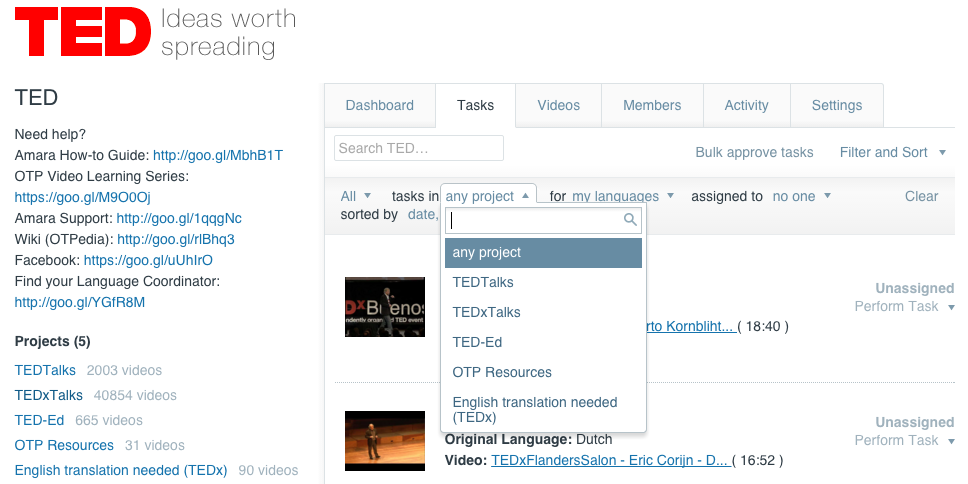
\includegraphics[width=0.7\textwidth]{textual/Figuras/TEDteamprojects.png}
        \caption{TED Teams project platform (Source: \href{https://translations.ted.com/How_to_Tackle_a_Review}{Wikipedia}).}
        \label{fig: ted-team-project}
        \end{figure}
        
    \item[TED2013:] This is a separate parallel corpus of TED Talks subtitles provided by CASMACAT\footnote{\href{http://www.casmacat.eu/corpus/ted2013.html}{http://www.casmacat.eu/corpus/ted2013.html}}, as described in~\textcite{tiedemann-2012-parallel}. The original source of the files is WIT$^3$\footnote{\href{https://wit3.fbk.eu}{https://wit3.fbk.eu}}, which stands for \emph{Web Inventory of Transcribed and Translated Talks}. WIT$^3$ is a ready-to-use version for research purposes of the multilingual transcriptions of TED Talks. The original dateset comprises a total of 346,643 segments, with approximately 5.5 million English tokens and 5.2 million Portuguese tokens. Notably, these transcripts were also translated by volunteers into various languages.
\end{description}


\section{Data Pre-processing and Compilation}

The TED Talks datasets selected for analysis were originally downloaded in TMX (Translation Memory eXchange). While TMX is a common format for storing translations, it was not directly usable for our purposes. To make the data more suitable for manipulation and further analysis, we developed a custom Python script leveraging the \texttt{Pandas}\footnote{\href{https://pandas.pydata.org}{https://pandas.pydata.org}} library. 

This script streamlines the conversion process by offering several key functionalities:

\begin{description}
    \item[DataFrame Structure:] We transformed data from TMX format into a Pandas DataFrame. This format is ideal for data manipulation, analysis, and integration with other Python libraries.
    \item[Large File Handling:] We identified and split large TMX files exceeding a user-defined size threshold into smaller chunks for efficient processing, preventing memory issues.
    \item[Metadata Preservation:] We preserved metadata from the original files by setting the \texttt{metadata=True} argument in the \texttt{clean\_data\_loader} function. This can be valuable for understanding the context and origin of the translation data.
    \item[Unique Data Point Identification:] We added an \texttt{inner\_id} column to the DataFrame, providing a unique identifier for each data point within the final CSV file. This facilitates tracking data points and merging datasets if necessary.
\end{description}

To illustrate the TMX conversion process, consider the following example from our corpus highlighting how the script transforms data from a less user-friendly XML format (TMX) into a structured and analyzable format (Pandas DataFrame):

\begin{verbatim} 
<tuv xml:lang="en">
  <seg> Put yourselves in my position. </seg>
</tuv>
<tuv xml:lang="pt">
  <seg> Coloquem-se no meu lugar! </seg>
</tuv>
\end{verbatim}


This snippet shows a portion of a TMX file containing a translation unit (TU) with two segments (seg). The first segment is in English (``Put yourselves in my position.''), and the second segment is its Portuguese translation (``Coloquem-se no meu lugar!'').

\begin{table}[htb]
\small
\centering
\begin{tabular}{|c|p{3cm}|p{3cm}|c|p{3cm}|}
\hline
\centering
{\textbf{lang\_pair}} & {\textbf{source}} & {\textbf{target}} & \textbf{inner\_id} & \textbf{produced\_from} \\ \hline\hline
en\_pt\_br & Put yourselves in my position. & Coloquem-se no meu lugar! & 4 & SRC\_TM\_DATA/ data\_2024/en-pt-2\_br.tmx \\ \hline
\end{tabular}
\caption{Example of Pandas DataFrame (after TMX conversion).}
\label{tab:example-pandas}
\end{table}

Table~\ref{tab:example-pandas} displays a portion of the resulting Pandas DataFrame after processing the TMX file. Each row represents a translation unit (TU). The DataFrame includes columns for the source sentence, target sentence, source language code, target language code, and potentially additional metadata preserved from the original file. An ``inner\_id'' column is also added for unique identification within the DataFrame.


\subsection{Data Cleaning and Normalization Steps}

This section details the data cleaning process applied to prepare the TED Talks transcript data for NMT engine training and evaluation. Following the initial conversion to a Pandas DataFrame, the cleaning steps aimed to ensure data quality and consistency for an effective analysis.

\begin{description}
    \item[Project Organization:] A well-structured project directory with subdirectories for each pre-processing stage was created to facilitate data organization and tracking throughout the cleaning pipeline.
    \item[Basic Cleaning Functions:] 
    \begin{description}
        \item[Missing Values \& Extraneous Markup Removal:] Rows containing missing entries (null values) and any residual HTML tags or code snippets were removed. Common parsers like \texttt{lxml}\footnote{\href{https://lxml.de}{https://lxml.de}}, \texttt{html.parser}\footnote{\href{https://docs.python.org/3/library/html.parser.html}{https://docs.python.org/3/library/html.parser.html}}, and \texttt{html5lib}\footnote{\href{https://pypi.org/project/html5lib/}{https://pypi.org/project/html5lib/}} were used for efficient HTML tag removal.
        \item[Duplicate Removal:] Identical entries in the dataset, potentially arising from data collection or processing errors, were removed to ensure each data point represents a unique translation pair.
        \item[Emoji Removal:] A custom function was implemented to identify and remove rows containing emojis, as they may not translate well using NMT engines.
    \end{description}
    \item[Targeted Cleaning:]
    \begin{description}
        \item[Incomplete Sentence Removal:] Sentences starting with punctuation marks in either source or target languages were removed, as they may represent incomplete phrases and hinder the translation process.
        \item[Strange Pattern Removal:] Unwanted strange text patterns were identified and removed using regular expressions (\texttt{re}\footnote{\href{https://docs.python.org/3/library/re.html}{https://docs.python.org/3/library/re.html}} library). This addressed noise or repetitive phrases that could also hinder the translation analysis.
        \item[Length Filtering:] Sentences outside a specific word and/or character range were excluded from the dataset to ensure reasonably manageable content size for NMT processing. This filtering included:
        \begin{description}
            \item \textbf{Token-based} (min: 4, max: 200): Sentences within this specific range of words/punctuation marks were retained.
            \item \textbf{Character-based} (min: 200, max: 450): Sentences within this specific range of characters (including punctuation marks) were retained.
            \item \textbf{Character-based Proportion} (lower: 0.001, upper: 0.999): Character proportions were calculated and mismatches in length between source and target texts were filtered out for better aligned translations.
        \end{description}
        \item[Repetition Removal:] Segments with excessively repetitive terms were removed, as they may not provide valuable data for the NMT engine.
        \item[Language Detection:] The \texttt{FastText}\footnote{\href{https://fasttext.cc/docs/en/python-module.html}{https://fasttext.cc/docs/en/python-module.html}} model identified languages within the data segments. Any segments in a language different from the source (English) and target (Portuguese) languages were filtered out.
        \item[Identical Text Removal:] Segments where source and target texts were exactly the same were deleted, as they do not represent actual translations.
        \item[Rare Characters Removal:] Rare characters with very low occurrence counts were identified and any segments containing them were removed to avoid introducing noise from infrequent characters (see Appendix~\ref{app:1} for examples).
        \end{description}
    \item \textbf{Extra Cleaning}:
    \begin{description}
        \item[Duplicate Removal (Recheck):] An additional check for duplicate entries was performed to ensure all duplicates were removed after the previous steps.
        \item[LaBSE Scoring:] LaBSE\footnote{\href{https://blog.research.google/2020/08/language-agnostic-bert-sentence.html}{https://blog.research.google/2020/08/language-agnostic-bert-sentence.html}} (Language-agnostic BERT Sentence Embedding), a multilingual sentence embedding model, was be used to calculate estimates of translation quality. Segments with LaBSE scores below a specific threshold were dropped to focus on higher-quality translations.
    \end{description}
    \item[Statistics Report:] A table summarizing the different types of deleted segments and their counts (from highest to lowest) was generated. This report provided insights into the cleaning process effectiveness and the quality of the original data.
\end{description}


\subsection{Refining the Dataset for NMT Testing and Evaluation}

This section details the multi-step process of filtering our data to create an optimal dataset for NMT engine evaluation, initially dividing the files into training and testing sets. However, despite a few attempts to build a custom NMT model using the Seq2Seq\footnote{\href{https://www.tensorflow.org/text/tutorials/nmt\_with\_attention}{https://www.tensorflow.org/text/tutorials/nmt\_with\_attention}} approach, our model resulted in subpar performance due to insufficient computational resources, time constraints, and the complexity of replicating the NMT task. Consequently, we decided to pursue the evaluation approach, which will be discussed in a later section.


\subsubsection{Further Refinement Steps}

To ensure the test set aligned with common translation scenarios while reflecting the focus of our research on spatial prepositions, we implemented the following filters:

\begin{description}
    \item[Sentence Segmentation:] We excluded entries containing multiple sentences, as NMT engines typically handle sentences individually.
    \item[Minimum Length:] Segments deemed too short were also removed, focusing on translations with a minimum required complexity.
    \item[Formatting:] Entries that began with a lowercase letter or lacked proper ending punctuation were also excluded to maintain consistency and well-formed structure.
    \item[Focus on Spatial Preposition:] Following our research goals of analyzing translations involving relevant spatial meanings, we prioritized sentences containing at least one of the prepositions: ACROSS, THROUGH, INTO, and ONTO.
\end{description}   

These additional filters reduced the initial dataset to a final size of $2,000$ segments, providing a more focused and effective test set for NMT engine testing and evaluation specific to spatial prepositions.

\section{Categorization by Meanings}

We employed a systematic approach to categorize prepositions in each EN source sentence based on their spatial and non-spatial meanings. This categorization is aligned with the definitions proposed by~\textcite{bruckfield2011prepositions} and entries found in the Cambridge Online Dictionary (CAM)\footnote{\href{https://dictionary.cambridge.org/}{https://dictionary.cambridge.org/}}. The specific categorizations are detailed in Table~\ref{tab:prep-categorizations}. 

\begin{table}[htb]
\small
\centering
\begin{tabular}{lp{.7\textwidth}}
\toprule
\textbf{EN Preposition} & \textbf{Meaning(s)}
\\ \midrule
Across  & \begin{tabular}[c]{@{}l@{}}(i) Perpendicular position; \\ (ii) Movement over a surface; \\ (iii) Opposite location; \\ (iv) Distribution; \\ (v) Non-spatial \end{tabular} \\
\hline
Into & \begin{tabular}[c]{@{}l@{}}(i) Movement or direction leading to enclosure; \\ (ii) Movement resulting in physical contact or collision; \\ (iii) Non-spatial \end{tabular} \\
\hline
Onto & \begin{tabular}[c]{@{}l@{}}(i) Movement to a location on a surface; \\ (ii) Sense of attachment; \\ (iii) Non-spatial \end{tabular} \\
\hline
Through & \begin{tabular}[c]{@{}l@{}}(i) Movement within a passage or conduit; \\ (ii) Movement within an open area, region, or place; \\ 
(iii) Movement past or penetrating a barrier;  \\ (iv) Part of a route; \\ (v) Non-spatial
\end{tabular} \\
\bottomrule  
\end{tabular}
\caption{Categorization of ACROSS, THROUGH, INTO, and ONTO (adpated from \textcite{bruckfield2011prepositions} and CAM).}
\label{tab:prep-categorizations}
\end{table}

Here are three examples of source sentences containing the preposition ACROSS included in this test set after the final filtering:

\ex. I woke up, they opened the door, I went out to get some fresh air, and I looked, and there was a man running \emph{across} $^{\textsuperscript{ii}}$ the runway. (\texttt{inner\_id: 30}) \label{ex: across-2}

Explanation: The superscript \emph{ii} corresponds to the specific meaning Across(ii) in Table~\ref{tab:prep-categorizations}, which refers to ``Movement over a surface.''

\ex. And so then Tarja was sitting \emph{across} $^{\textsuperscript{iii}}$ the table from me. (\texttt{inner\_id: 3011154}) \label{ex: across-3}

Explanation: The superscript \emph{iii} corresponds to the specific meaning Across(iii) in Table~\ref{tab:prep-categorizations}, which refers to ``Opposite location.''

\ex. In the mid-19th century, suspension bridges were collapsing all \emph{across} $^{\textsuperscript{iv}}$ Europe. (\texttt{inner\_id: 343660}) \label{ex: across-4}

Explanation: The superscript \emph{iv} corresponds to the specific meaning Across(iv) in Table~\ref{tab:prep-categorizations}, which refers to ``Distribution.'' 

Examples~\ref{ex: across-2}, \ref{ex: across-3} and \ref{ex: across-4} showcase the variety of contexts for ACROSS, as summarized in Table~\ref{tab:prep-categorizations}. These examples allow for a more nuanced evaluation of NMT engines' ability to capture the subtleties of spatial prepositions during translation.


\section{The Translation Process}

To ensure reproducibility, we prioritized freely available resources for translating our test set across different platforms. These resources included Python libraries, APIs, and open-source language models. However, limitations like request quotas and character restrictions necessitated the development of alternative strategies (details provided later).

\subsection{NMT Systems}

We employed three established NMT service providers for our evaluation:

\subsubsection{Google Translate}

To translate using Google Translate, we employed the \texttt{googletrans}\footnote{\href{https://pypi.org/project/googletrans/}{https://pypi.org/project/googletrans/}} a free and open-source Python library, to leverage Google Translate Ajax API. This library allows users to translate text directly within their Python code, utilizing the same servers that power translate.google.com.

\subsubsection{DeepL Translator}

Due to limitations on free access, we utilized a combination of resources for DeepL:

\begin{description}
    \item[\hspace{=2em}Rapid API]\footnote{\href{https://rapidapi.com/splintPRO/api/deepl-translator/}{https://rapidapi.com/splintPRO/api/deepl-translator/}}: This server provided programmatic access with limited requests per minute.
    \item[\hspace{=2em}DeepL Console]\footnote{\href{https://www.deepl.com/en/translator}{https://www.deepl.com/en/translator}}: Offered a web interface for manual translations, but with limitations on the number of translated tokens.
    \item[\hspace{=2em}DeepL Desktop App] (installed on a Macbook Pro Late 2013 -- see Figure~\ref{fig: deepl-app}): Facilitated offline translation capabilities, allowing us to translate larger batches.
\end{description}



For efficiency, the test set was translated in batches of 50 sentences each. All DeepL translations were then compiled into a single file for further analysis. 

\begin{figure}[htb]
\centering
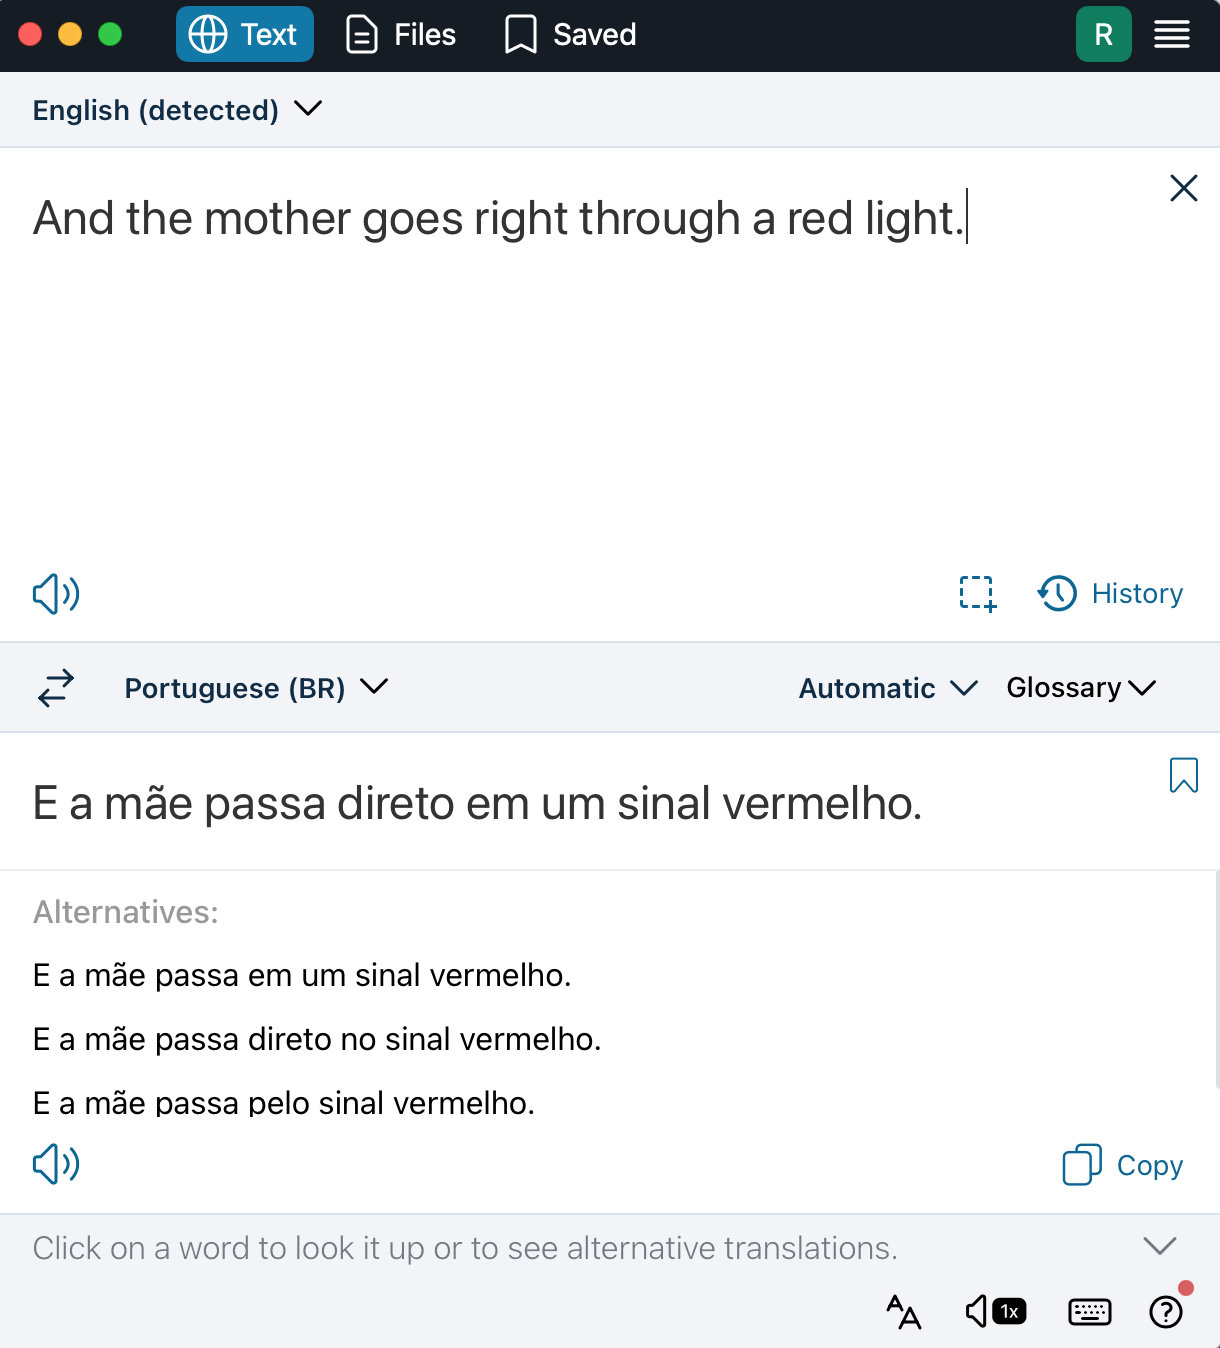
\includegraphics[width=0.6\textwidth]{textual/Figuras/deepl-app.png}
\caption{DeepL Translator app interface (Source: Our own).}
\label{fig: deepl-app}
\end{figure}

\subsubsection{Amazon Translate}

We utilized Amazon's  console\footnote{\href{https://console.aws.amazon.com/translate/home}{https://console.aws.amazon.com/translate/home}} and a free AWS account for the translation taks.

\begin{description}
    \item[\hspace{=2em}Amazon (Stock):] We leveraged the free Batch translation service to translate the 2,000-segment test set from a single CSV file.
    \item[\hspace{=2em}Amazon (Custom):] We trained a custom model using the parallel data option on Amazon Translate with the remaining 344,643 segments from the training set. This allowed us to explore the impact of model customization on translation quality.
\end{description}


\subsection{LLMs}

To perform machine translations using LLMs, we utilized the Python library \texttt{Ollama} \footnote{\href{https://github.com/ollama/ollama-python}{https://github.com/ollama/ollama-python}}, which facilitates running open-source generative models locally or on the cloud through \texttt{LangChain}\footnote{\href{https://api.python.langchain.com/en/latest/community_api_reference.html}{https://api.python.langchain.com/en/latest/community\_api\_reference.html}}. This allowed us to explore the capabilities of LLMs for translation tasks. However, it is important to note that the computational demands of LLMs required the use of Google Colab Pro with its enhanced GPUs for efficient processing.

\subsubsection{Meta's LLaMa}

We experimented with three variations of the  open-source LLaMa family:

\begin{description}
\item[\hspace{=2em}LLaMa 3 (8B)]\footnote{\href{https://huggingface.co/meta-llama/Meta-Llama-3-8B}{https://huggingface.co/meta-llama/Meta-Llama-3-8B}}: As of the date of this work, this is the latest generation of LLaMa. It adopts a decoder-only transformer architecture and employs a tokenizer with a vocabulary of 128K tokens, facilitating more efficient language encoding. Throughout training, the model processes sequences of 8,192 tokens while utilizing a mask to prevent self-attention from extending beyond document boundaries. Trained on a dataset of 15 trillion tokens, it stands as the most advanced LLaMa model to date, featuring an 8K context length—twice that of LLaMa 2. This significant advancement is reinforced by over 5\% non-English pretraining data, covering more than 30 languages~\parencite{llama3}.    \item[\hspace{=2em}LLaMa 2 Uncensored]\footnote{\href{https://huggingface.co/georgesung/llama2_7b_chat_uncensored}{https://huggingface.co/georgesung/llama2\_7b\_chat\_uncensored}}: This uncensored version, developed by George Sung and Jarrad Hope and based on Meta's open-source Llama 2, underwent training on 2 trillion tokens. With 7 billion parameters and a size of 3.8GB, this model was pretrained on publicly available online data sources. Its architecture follows the decoder-only variant of transformers and employs a tokenizer with a vocabulary of 128K tokens, which is 40\% larger than LLaMa 1. Notably, this model offers unrestricted outputs, distinguishing it from the original Llama 2 and making it suitable for various applications \parencite{llama2}.
    \item[\hspace{=2em}LLaMa 2 (13B)]\footnote{\href{https://huggingface.co/meta-llama/Llama-2-13b}{https://huggingface.co/meta-llama/Llama-2-13b}}: The 13B Llama 2 boasts a larger size (13B parameters) compared to the 7B version. This increase suggests potential for capturing more complex language patterns, which could lead to potentially improved performance in various tasks. Both models likely utilize the same decoder-only transformer architecture, excelling at text generation. However, information on the 13B's output limitations is currently unavailable. Further testing  is needed to definitively determine any performance advantage the 13B model holds over the 7B version \parencite{llama2}.
\end{description}

 
\subsubsection{Google's Gemma}

We examined Gemma 7B \parencite{gemma_2024, gemma}, a lightweight open-source language model from Google, built using technology similar to Gemini models. It is a text-to-text, decoder-only large language models, available in English, possessing open weights, pre-trained variants, and instruction-tuned variants. It was trained on a dataset of 6 trillion tokens and a context length of 8192 tokens. The specific composition of this data is not publicly available. Gemma excells in tasks such as text generation, question answering, summarization, and reasoning, and can be fine-tuned for other tasks.


\subsubsection{Mistral Models}

We also investigated two open-source models by Mistral AI:

\begin{description}
    \item[\hspace{=2em}Mixtral-8x7B (47B)]\footnote{\href{https://huggingface.co/mistralai/Mixtral-8x7B-v0.1}{https://huggingface.co/mistralai/Mixtral-8x7B-v0.1}}: Mixtral, a decoder-only language model, leverages a sparse mixture-of-experts network for cost-efficiency. Trained on publicly available web data \parencite{mixtral}, Mixtral employs a similar architecture to Mistral 7B, but with each layer utilizing 8 expert blocks. This approach allows access to a larger parameter pool (47 billion) while actively using only a portion (13 billion) during inference, leading to cost savings. Additionally, Mixtral boasts a large context window (32k tokens) and native multilingual capabilities (English, French, German, Spanish, Italian). This combination positions Mixtral as a strong contender for various NLP tasks \parencite{jiang2024mixtral}.
    \item[\hspace{=2em}Mistral (7B) Instruct v0.2]\footnote{\href{https://huggingface.co/mistralai/Mistral-7B-Instruct-v0.2}{https://huggingface.co/mistralai/Mistral-7B-Instruct-v0.2}}: Mistral 7B is a decoder-only 7-billion parameter, open-source language model (LLM) achieving competitive performance on various benchmarks \parencite{mistral, jiang2023mistral}. It employs grouped-query attention (GQA) and sliding window attention (SWA) for efficient text processing, particularly for handling long sequences. Mistral 7B's adaptability allows it to generate responses based on instructions and predict missing text, making it suitable for tasks like chatbots and content generation.
    \end{description}

To collect the translations, two zero-shot prompt variations were used:

\newtcolorbox{promptbox}{
colback=gray!5,
arc=4pt,
left skip=5pt,
right skip=5pt,
boxsep=5pt,
fonttitle=\bfseries,
boxrule = 0pt,
toprule = 4.5pt,
enhanced,
fuzzy shadow = {0pt}{-2pt}{-0.5pt}{0.5pt}{black!35},
width=\textwidth,
title=Standard Prompt:
}

\begin{promptbox}
context  $=$ ``You are a professional translator.'' \\
task $=$ ``Translate the following sentence from English to Portuguese: \textbf{[source\_text]}'' 
\end{promptbox}

\newtcolorbox{promptbox1}{
colback=gray!5,
arc=4pt,
left skip=5pt,
right skip=5pt,
boxsep=5pt,
fonttitle=\bfseries,
boxrule = 0pt,
toprule = 4.5pt,
enhanced,
fuzzy shadow = {0pt}{-2pt}{-0.5pt}{0.5pt}{black!35},
width=\textwidth,
title=Alternative Prompt:
}

\begin{promptbox1}
context  $=$ ``You are a professional translator.'' \\
task $=$ ``Translate the following sentence from English to Portuguese: \textbf{[source\_text]}. Provide only ONE translation. DON'T add any additional comments, observations or translations.''
\end{promptbox1}


\section{The Scoring Step}

This section details the subsequent scoring process for translation quality evaluation, after data collection and post-editing. We utilized Python libraries to calculate these scores for each data point.


\begin{description}
    \item[NLTK:] Both BLEU and METEOR scores were calculated using the \texttt{nltk}\footnote{\href{https://www.nltk.org}{https://www.nltk.orgl}} library, which handles text tokenization (splitting sentences into words) as a pre-processing step. The \texttt{nltk.translate} submodule provides functions for calculating:
    \begin{description}
        \item[BLEU score:] \texttt{bleu\_score}\footnote{\href{https://www.nltk.org/api/nltk.translate.bleu_score.html}{https://www.nltk.org/api/nltk.translate.bleu\_score.html}} with \texttt{SmoothingFunction().method1} focuses on \emph{n}-gram (sequence of \emph{n} words) overlaps between the reference and translated text, with adjustments for cases with missing values in the translation.
        \item[METEOR score:] \texttt{meteor\_score}\footnote{\href{https://www.nltk.org/api/nltk.translate.meteor_score.html}{https://www.nltk.org/api/nltk.translate.meteor\_score.html}} considers factors like unigram precision, recall, synonym matching, and stemming to assess translation quality. 
    \end{description}
    \item[SacreBLEU:] TER scores were calculated using the \texttt{sentence\_ter} function from the  \texttt{sacrebleu}\footnote{\href{https://github.com/mjpost/sacrebleu/tree/master}{https://github.com/mjpost/sacrebleu/tree/master}} library. It measures the number of edits (insertions, deletions, substitutions) required to transform the translated text into the reference text.
    \item[Transformers:] We calculated BERTScores to assess semantic similarity between reference and translated texts utilizing the \texttt{transformers} library to load a pre-trained BERT model and tokenizer\footnote{\href{https://huggingface.co/transformers/v3.0.2/model_doc/bert.html}{https://huggingface.co/transformers/v3.0.2/model\_doc/bert.html}}. BERT works by generating sentence embeddings, which capture the meaning of a sentence in a high-dimensional space. We calculate the cosine similarity between these embeddings to determine how close the semantics of the reference and translated text are.
    \item[Cometml:] The \texttt{cometml}\footnote{\href{https://pypi.org/project/comet-ml/}{https://pypi.org/project/comet-ml/}} library was used to load the pre-trained COMET model named ``Unbabel/wmt22-comet-da''. This model is specifically designed for evaluating translation quality, focusing on aspects like fluency, adequacy, and coherence. We formatted our data to match the model's input requirements and then retrieved the score based on the model's prediction.
\end{description}


\section{Score Distributions and Confidence Intervals}

To analyze the distribution of scores across models, box plots were utilized, offering a visual summary of the data's key statistics: minimum, first quartile (Q1), median, third quartile (Q3), and maximum. Additionally, confidence intervals (CIs) were computed at a 95\% confidence level to estimate the likely range of the true difference between the means of compared systems, based on the calculated means \parencite{zhang-vogel-2004-measuring}. This approach facilitated an understanding of the precision among models and statistical significance. Refer to Figures \ref{fig:boxplot} and \ref{fig:ci} for visual representations of these steps.

For these analyses, the following Python libraries for statistical computations were employed: \texttt{NumPy}\footnote{\href{https://numpy.org}{https://numpy.org}} for numerical operations, including functions for median, quartiles, percentiles, mean, and standard deviation; and \texttt{SciPy}\footnote{\href{https://scipy.org}{https://scipy.org}} for statistical functions such as \texttt{stats.t.interval} to calculate CIs.

\begin{figure}[htb]
\centering
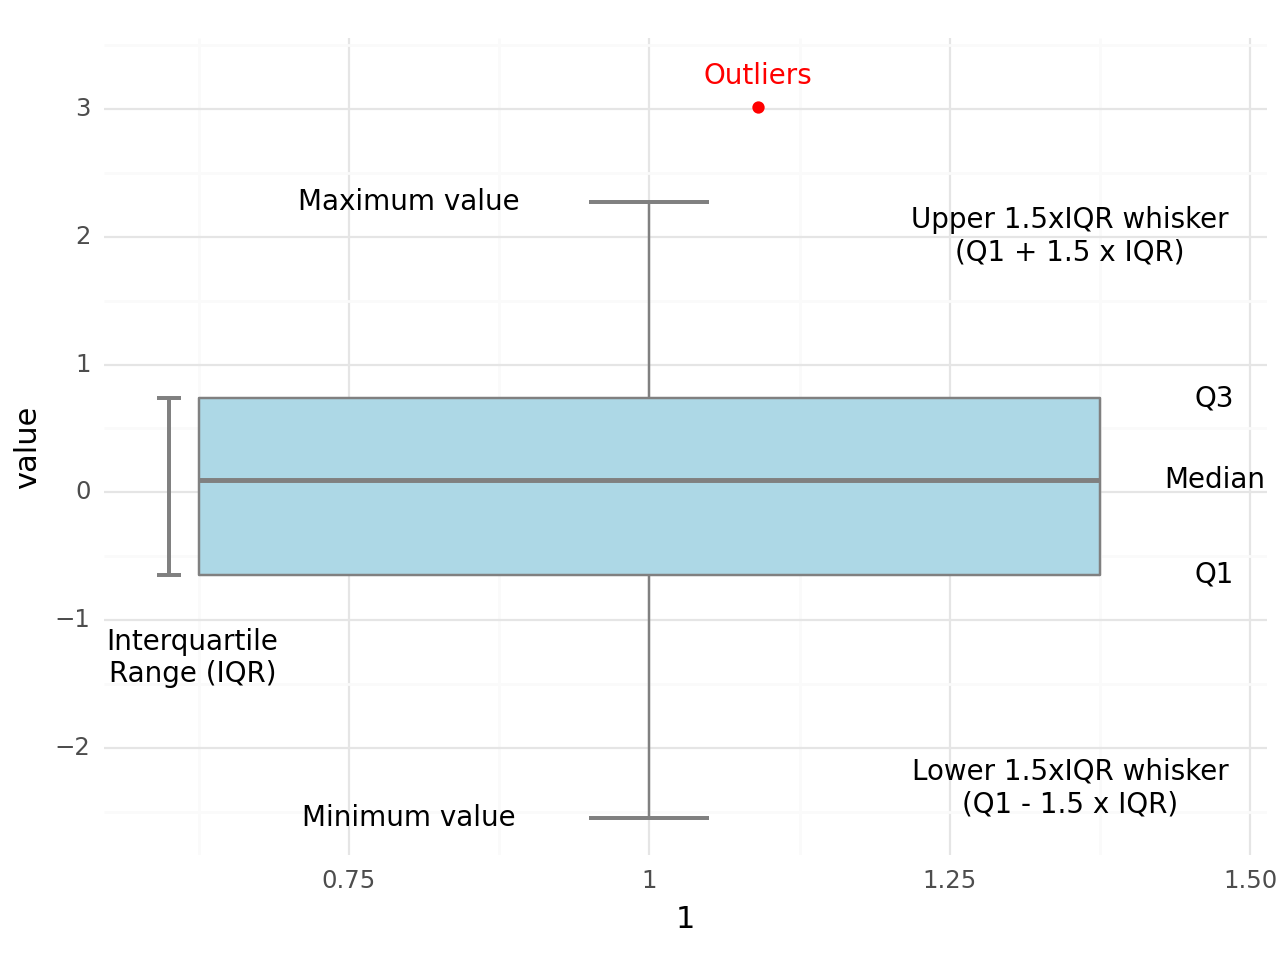
\includegraphics[width=.8\textwidth]{textual/Figuras/boxplot-real.png}
\caption{Key Features of Box Plot (Source: Our own).}
\label{fig:boxplot}
\end{figure}

Key features of the boxplot:

\begin{description}
    \item[Minimum Value:] The lowest score, excluding outliers (shown at the end of the bottom whisker).
    \item[Lower Quartile:] Twenty-five percent of scores fall below the lower quartile value (also known as the first quartile).
    \item[Median:] The median marks the mid-point of the data and is shown by the line that divides the box into two parts (sometimes known as the second quartile). Half the scores are greater than or equal to this value, and half are less.
    \item[Upper Quartile:] Seventy-five percent of the scores fall below the upper quartile value (also known as the third quartile). Thus, 25\% of data are above this value.
    \item[Maximum Value:] The highest score, excluding outliers (shown at the end of the top whisker).
    \item[Whiskers:] The upper and lower whiskers represent scores outside the middle 50\% (i.e., the lower 25\% of scores and the upper 25\% of scores).
    \item[Interquartile Range (IQR):] The box plot shows the middle 50\% of scores (i.e., the range between the 25th and 75th percentile).
    \item[Outliers:] Individual data points that fall outside the whiskers and are typically considered as extreme values.
\end{description}

The quartiles (Q1 and Q3) and the interquartile range (IQR) were calculated using the \texttt{np.percentile} function from \texttt{NumPy}. The whiskers were then determined by extending from the quartiles by 1.5 times the IQR, ensuring that they include the most extreme non-outlier data points within that range.

\begin{figure}[htb]
\centering
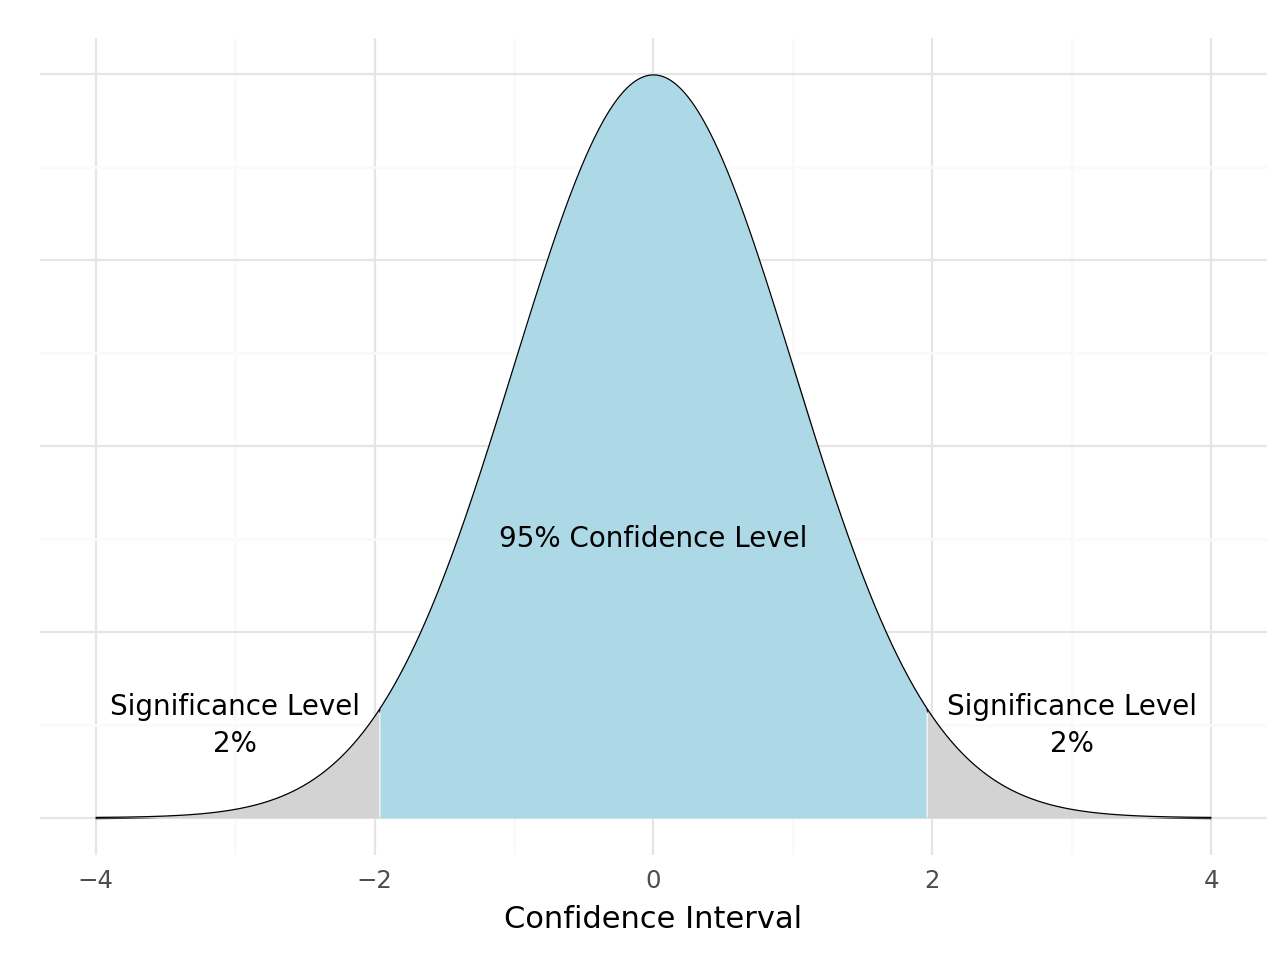
\includegraphics[width=.6\textwidth]{textual/Figuras/confidence-intervals.png}
\caption{Confidence Intervals (CIs) (Source: Our own).}
\label{fig:ci}
\end{figure}


To calculate CIs, we used the \texttt{stats.t.interval} function from the \texttt{scipy.stats} module. This function employs the Student’s t-distribution to compute the interval for a specified confidence level. The probability density function (pdf) is given by:

\begin{equation} \label{formula: t-dis}
f(x|df) = \frac{\Gamma\left(\frac{df+1}{2}\right)}{\sqrt{\pi df} \, \Gamma\left(\frac{df}{2}\right)} \left(1 + \frac{x^2}{df} \right)^{-\frac{df+1}{2}}
\end{equation} 

where $x$ is a real number, $df$ represents the degrees of freedom parameter and $\Gamma$ is the gamma function \parencite{scipy_stats_t}. The parameters utilized in this function include:

\begin{description}
    \item[Confidence Level (0.95):] Specifies the probability that the calculated interval contains the true population parameter, typically set to 95\%.
    \item[Degrees of Freedom:] Determined by the sample size, calculated as the number of observations minus one.
    \item[Location Parameter] (\texttt{mean\_score}): Represents the mean of the distribution, serving as the center around which the interval is constructed.
    \item[Scale Parameter] (\texttt{stats.sem(filtered\_scores)}): Estimates the standard deviation of the sample mean, used to scale the interval width.
\end{description}


After specifying these parameters, the \texttt{stats.t.interval} function computes the CI and returns the lower and upper bounds of the interval.

\section{Human Evaluation Process}
\label{sec: Human Evaluation}

This section outlines the systematic approach used to evaluate translation quality using human reviews and manual error classification. The goal was to accurately assess model performance and ultimately identify areas for improvement in translation quality.

At this stage, it is worth noting that not all models from the previous step were selected for manual analysis. Instead, we focused on comparing LLM performace against traditional NMT systems. To this end, we conducted a comprehensive analysis of all LLMs, comparing them against each other and against the top NMT performer from the scoring stage. This comparison aimed to validate the accuracy of the scores and confirm whether there was real statistical significance in performance between the two groups.

\subsection{Data Reduction for Human Review}
To gain a deeper understanding of translation quality, we employed a two-step process to select a representative sample for human reviews:

\begin{description}
\item[Random Selection:] We initially selected a reduced representative sample comprising 200 segments (10\% of the total 2,000 translated segments) for human evaluation. This process was designed to ensure randomness and diversity within the sample. We shuffled 500 segments using the Pandas' \texttt{sample}\footnote{\href{https://pandas.pydata.org/pandas-docs/stable/reference/api/pandas.DataFrame.sample.html}{https://pandas.pydata.org/pandas-docs/stable/reference/api/pandas.DataFrame.sample.html}} function.
\item[Subset Curation:] From the initially shuffled pool, human judgment was employed to review the segments and curate a refined subset of 200 segments to undergo human reviews. This approach ensured a sufficient sample size encapsulating a variety of errors for thorough analysis.
\end{description}


\subsection{Manual Error Classification}
\label{subsec: Manual Error Classification}

In this step, each translated segment underwent a meticulous manual error classification process to identify and categorize translation errors accurately, comprehensively, and efficiently. The error classification scheme, organized into two main categories, is detailed in Table~\ref{tab: error_categories}. This scheme was utilized to systematically identify and categorize errors, enabling a more precise, nuanced, and reliable assessment of model performance.

\begin{table}[htb]
\centering
\small
\begin{tabular}{lp{.5\textwidth}}
\toprule
\textbf{Annotations} & \textbf{Description} \\
\midrule
\quad Correct (cc) & Accurate translation. \\
\midrule
\quad \textbf{Spatial Errors} & \\
\quad \quad Polysemy (po) & Incorrect polysemous prepositional sense. \\
\quad \quad Syntactic Projection (sp) & Incorrect copy of source language syntax.  \\
\quad \quad Wrong Sense (ws) & Incorrect unrelated prepositional sense. \\
\midrule
\quad \textbf{Non-Spatial Errors} &  \\
\quad \quad Idiomatic Expression (ie) & Mistranslation of phrasal verbs or idioms. \\
\midrule
\quad \textbf{Other Errors} &  \\
\quad \quad Addition (ad) & Unnecessary added words/phrases.  \\
\quad \quad Agreement (ag) & Wrong subject-verb/noun combinations.  \\
\quad \quad Anglicism (ag) & Directly borrowed English structure.  \\
\quad \quad Collocation (co) & Incorrect verb combinations.  \\
\quad \quad Grammar/orthography (gr) &  Grammar/spelling errors.  \\
\quad \quad Interlanguage/code-switching (in) & Mixed use of target and/or other languages.  \\
\quad \quad Omission (om) & Missing words/phrases from source text.\\
\quad \quad Untranslated (un) & Source text not (fully or partly) translated. \\
\quad \quad Wrong Lexical Choice (wl) & Inappropriate noun choice. \\
\quad \quad Wrong Verb Mood/Tense (wt) & Incorrect verb mood/tense. \\
\bottomrule
\end{tabular}
\caption{Error Annotation Scheme.}
\label{tab: error_categories}
\end{table}


During the manual error classification step, each automatic translation was analyzed primarily focusing on fluency in the target language, paying occasional attention to the reference and source texts for specific types of errors. This approach facilitated an evaluation centered on the quality of the system itself and its generated output. Error types were then annotated in an additional column in the dataset for individual records.

Given that mistranslation is a broad category, in this research, we are particularly
interested in identifying four specific mistranslation errors involving prepositions:

\begin{description}
    \item[Polysemy:] These errors happen when the MT system picks the wrong meaning 
    for a polysemous preposition (with multiple 
    meanings, spatial or not). Prepositions can be tricky because their meaning depends on the context. In spatial semantics, an MT system might misinterpret the 
    meaning of a preposition in the source language, leading to an inaccurate expression in the target language. An example is translating ``a barricade across the door'' to ``uma barreira do outro lado da porta'' (on the other side of the door) in PT-br instead of ``uma barricada atravessada na porta.'' ``Atravessada'' (crossing) is more fitting in this context.
    
    \item[Syntactic Projection:] Typically an extension of polysemy, these errors occur when the MT system not only mistranslates the preposition's meaning but also directly copies the syntax (word order) from the source language to the target language. This violates the target language's rules for expressing spatial relationships, creating problems because languages express spatial relationships differently~\parencite{talmy2000toward, talmy2000towardb, slobin2005relating}. For example, the EN phrase ``to swim across the river'' (using a Manner verb and a Path preposition) requires a different grammatical construction in PT-br, such as ``atravessar o rio nadando'' (literally ``to cross the river by swimming''). A common mistranslation of this sort would be to translate the phrase as ``nadar do outro lado do rio'', as illustrated in~\textcite{fernandes-etal-2024-spatial}. 
    
    \item[Wrong Sense Errors:] These errors occur when a spatial preposition is mistranslated into a grammatically correct but semantically %M: incorrect
    incorrect
    preposition in the target language. This mismatch arises because the chosen preposition does not accurately convey any of the possible spatial meanings of the original polysemous preposition in case. For instance, translating ``The store across the street'' as ``A loja através da rua'' in PT-br results in a wrong sense error. While ``através'' can mean ``through,'' it does not correctly convey the idea of an opposite location, which ``do outro lado da rua'' (on the other side of the street) would accurately express.
    
    \item[Idiomatic Expressions:] The only non-spatial errors on the list, these typically occur when translating idiomatic phrases whose figurative meaning goes beyond the literal meaning of the individual words. Often, these expressions involve verbs and spatial prepositions, but their meaning is not necessarily spatial -- a key distinction from syntactic projection errors. For instance, translating ``to run through a list'' literally as ``correr pela lista'' (PT-br) would be a mistake. This focuses on the individual words (run + through) rather than the intended meaning, conveyed more accurately by ``ler rapidamente'' (to read quickly).
\end{description}

By employing this well-defined human evaluation process and error classification scheme, we were able to effectively assess the quality of the automatic translations and identify areas for model improvements. This comprehensive approach allowed us to compare the performance of LLMs against traditional NMT providers and confirm any statistically significant differences.


\subsection{Chi-Square Test} 
\label{sec: chi-test}

The Chi-Square ($\chi^2$) Test of Independence is a statistical method utilized to determine the association between two categorical variables. In this study, the Chi-Square test was employed using data from the human review step to validate the null hypothesis concerning the impact of spatial and non-spatial errors on the translations. The test was conducted in Python using the \texttt{chi2\_contingency}\footnote{\href{https://docs.scipy.org/doc/scipy/reference/generated/scipy.stats.chi2\_contingency.html}{https://docs.scipy.org/doc/scipy/reference/generated/scipy.stats.chi2\_contingency.html}} function from the \texttt{scipy.stats} module. Figure~\ref{fig:chi} illustrates the Chi-Square Distribution while Equation~\ref{chi-test} describes the Chi-Square test formula. The Chi-Square Test requires:

\begin{figure}[htb]
\centering
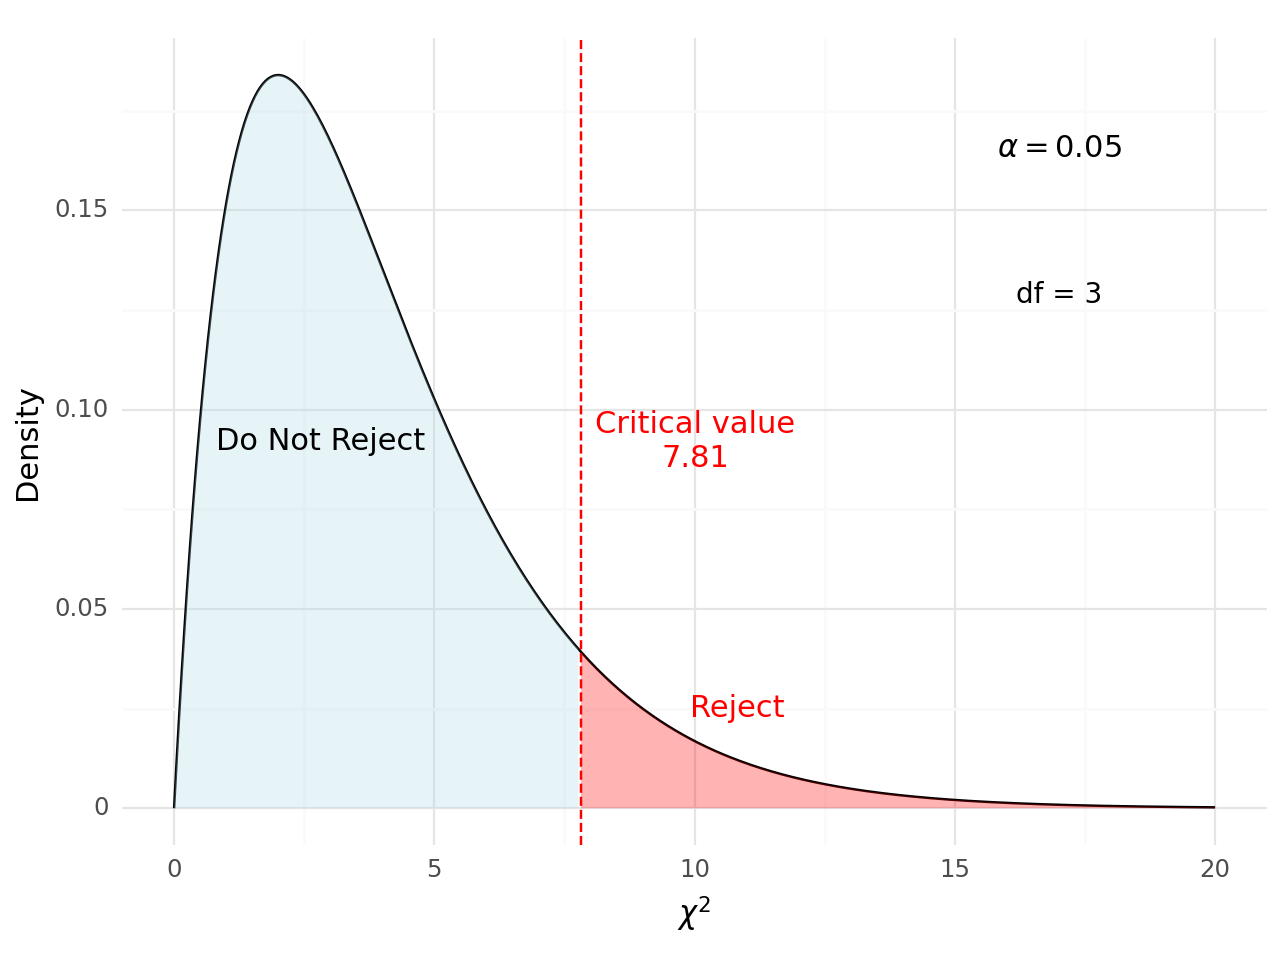
\includegraphics[width=.6\textwidth]{textual/Figuras/Results/chi.png}
\caption{Chi-Square ($\chi^2$) Distribution for $\alpha = 0.05$ and $df = 3$. (Source: Our own).}
\label{fig:chi}
\end{figure}


\begin{description}
    \item[Degrees of Freedom (df):] Depends on the number of categories or groups compared. Calculated as the number of observations minus one.
    \item[Significance Level ($\alpha$):] The probability of rejecting the null hypothesis when it is true, commonly set at $0.05$ (5\%).
    \item[Chi-Square Distribution:] Used to assess the goodness-of-fit or independence between categorical variables by comparing observed and expected frequencies.
    \item[Critical Value:] The threshold beyond which we reject the null hypothesis. For $df = 3$ and $\alpha = 0.05$, the critical value is $7.81$, obtained from chi-square distribution tables or statistical software.
    \item[\hspace{=2em}]Interpretation of the Critical Value:
    \begin{itemize}
    \item \textbf{$\chi^2 < 7.81$:} Fail to reject the null hypothesis. This indicates insufficient evidence to suggest a significant difference between observed and expected frequencies, implying that the observed data fits the expected distribution well.
    \item \textbf{$\chi^2 \ge 7.81$:} Reject the null hypothesis. This suggests a significant difference between observed and expected frequencies, indicating that the observed data does not fit the expected distribution well, thereby suggesting a possible relationship or effect.
\end{itemize}

\begin{equation} \label{chi-test}
    \chi^2_c = \sum \frac{(O_i - E_i)^2}{E_i}
\end{equation}

\hspace{=2em}In this formula, $c$ represents the degrees of freedom, and $O_i$ and $E_i$ are the observed and expected frequencies, respectively. If the calculated $\chi^2$ exceeds the critical value, the null hypothesis is rejected, indicating a significant difference between the observed and expected frequencies at the $0.05$ significance level.
\end{description}





The \texttt{chi2\_contingency} function from the \texttt{scipy.stats} module includes the following parameters and return values:

\begin{description}
    \item[Parameters] 
\end{description}
  
    \begin{itemize}
        \item \textbf{\texttt{observed} (array\_like):} The contingency table containing the observed frequencies (i.e., number of occurrences) in each category. In the two-dimensional case, the table is often described as an “R x C table”.
        \item \textbf{\texttt{correction} (bool, optional):} If \texttt{True}, and the degrees of freedom is 1, apply Yates’ correction for continuity. The effect of the correction is to adjust each observed value by 0.5 towards the corresponding expected value.
        \item \textbf{\texttt{lambda\_} (float or str, optional):} By default, the statistic computed in this test is Pearson’s chi-squared statistic. \texttt{lambda\_} allows a statistic from the Cressie-Read power divergence family to be used instead. See \texttt{scipy.stats.power\_divergence}\footnote{\href{https://docs.scipy.org/doc/scipy/reference/generated/scipy.stats.power\_divergence.html}{https://docs.scipy.org/doc/scipy/reference/generated/scipy.stats.chi2\_contingency.html}} for details. 
    \end{itemize}
    
\begin{description}
    \item[Returns] 
\end{description}  

    \begin{itemize}
        \item \textbf{\texttt{res} (Chi2ContingencyResult):} An object containing the following attributes:
        \begin{itemize}
            \item \textbf{\texttt{statistic} (float):} The test statistic.
            \item \textbf{\texttt{pvalue} (float):} The p-value of the test.
            \item \textbf{\texttt{dof} (int):} The degrees of freedom.
            \item \textbf{\texttt{expected\_freq} (ndarray):} The expected frequencies, based on the marginal sums of the table.
        \end{itemize}       
    \end{itemize}

\vspace{0.5em} % Adjust the value (e.g., 1em) to increase or decrease the gap

In Chapter~\ref{cap:Methods}, we outlined the methodology employed to explore spatial semantics in translation, comparing NMT systems and LLMs. These methods ensure a rigorous analysis of translation quality, focusing on the intricacies of spatial language. By establishing a robust framework for data collection and evaluation, this chapter lays a strong foundation for the subsequent discussion of results and their implications in MT studies.


